\documentclass[10pt]{article}
\usepackage{pstricks-add}
\usepackage{graphics}
\pagestyle{empty}
\begin{document}
\psset{xunit=1.0cm,yunit=1.0cm,algebraic=true,dotstyle=o,dotsize=3pt 0,linewidth=0.8pt,arrowsize=3pt 2,arrowinset=0.25}
\begin{pspicture*}(-0.35,1.39)(11.39,10.33)
\psline[linecolor=blue]{->}(5.87,8.56)(7.22,7.71)
\psline[linecolor=blue]{->}(7.22,7.71)(7.71,6.19)
\psline[linecolor=blue]{->}(7.11,4.71)(5.7,3.96)
\psline[linewidth=1.2pt,linecolor=red]{->}(5.7,3.96)(4.14,4.3)
\psline[linecolor=blue]{->}(4.14,4.3)(3.16,5.56)
\psline[linecolor=blue]{->}(3.22,7.16)(4.29,8.34)
\psline[linecolor=blue]{->}(4.29,8.34)(5.87,8.56)
\parametricplot[linewidth=1.2pt,linecolor=red]{4.114738681501859}{6.089610168092989}{1*0.92*cos(t)+0*0.92*sin(t)+6.22|0*0.92*cos(t)+1*0.92*sin(t)+4.72}
\psline[linewidth=1.2pt,linecolor=red]{->}(4.14,4.3)(7.11,4.71)
\begin{scriptsize}
\psdots[dotstyle=*](3.16,5.56)
\rput[bl](2.59,5.33){$u_{i+2}$}
\psdots[dotstyle=*](4.14,4.3)
\rput[bl](3.85,3.99){$u_{i+1}$}
\psdots[dotstyle=*](5.7,3.96)
\rput[bl](5.51,3.53){$u_i$}
\psdots[dotstyle=*](7.11,4.71)
\rput[bl](7.41,4.61){$u_{i-1}$}
\psdots[dotstyle=*](7.71,6.19)
\rput[bl](7.93,6.15){$u_3$}
\psdots[dotstyle=*](7.22,7.71)
\rput[bl](7.35,7.75){$u_2$}
\psdots[dotstyle=*](5.87,8.56)
\rput[bl](5.95,8.73){$u_1$}
\psdots[dotstyle=*](4.29,8.34)
\rput[bl](3.99,8.61){$u_k$}
\psdots[dotstyle=*](3.22,7.16)
\rput[bl](2.59,7.35){$u_{k-1}$}
\psdots[dotsize=1pt 0,dotstyle=x,linecolor=blue](7.62,5.72)
\psdots[dotsize=1pt 0,dotstyle=x,linecolor=blue](7.48,5.4)
\psdots[dotsize=1pt 0,dotstyle=x,linecolor=blue](7.32,5.08)
\psdots[dotsize=1pt 0,dotstyle=x,linecolor=blue](3.14,6.78)
\psdots[dotsize=1pt 0,dotstyle=x,linecolor=blue](3.08,6.4)
\psdots[dotsize=1pt 0,dotstyle=x,linecolor=blue](3.1,6.08)
\psdots[dotsize=5pt 0,dotstyle=triangle*,linecolor=red](7.11,4.55)
\end{scriptsize}
\end{pspicture*}


\begin{figure}
\centering
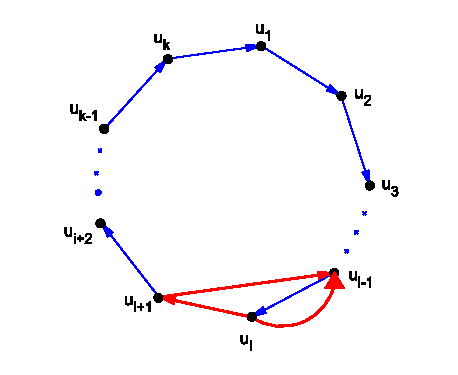
\includegraphics{imagen.eps}
\end{figure}
\end{document}

